This section reports the main empirical findings. Unless stated otherwise, results use WOMD \texttt{validation\_interactive} (12{,}800 scenarios), $K{=}6$, and Protocol~A. Protocol~A matches the operating proxy stack; Protocol~B, together with the conservative-activation cross-evaluation later in the section, is the more conservative reference for absolute compliance. We distinguish \emph{best-of-$K$} accuracy, which measures candidate-set coverage, from \emph{selected} accuracy, which measures the trajectory actually executed after selection.

%-------------------------------------------------------------------------------
\subsection{Trajectory Prediction Accuracy}
\label{subsec:trajectory_accuracy}
%-------------------------------------------------------------------------------

We begin with candidate-set accuracy, which establishes the upper bound on what any downstream selector can achieve. Table~\ref{tab:main_results} situates RECTOR's generation quality within the range of published methods.

\begin{table}[t]
\centering
\caption{Candidate-Set Accuracy Context on WOMD \texttt{validation\_interactive}}
\label{tab:main_results}
\begin{tabular}{lccc}
\toprule
\textbf{Method} & \textbf{minADE (m)} \color{green}{$\downarrow$} & \textbf{minFDE (m)} \color{green}{$\downarrow$} & \textbf{Miss (\%)} \color{green}{$\downarrow$} \\
\midrule
LaneGCN & 0.87 & 1.92 & 28.4 \\
DenseTNT & 0.73 & 1.55 & 20.1 \\
M2I & 0.75 & 1.63 & 22.8 \\
Wayformer & 0.68 & 1.42 & 18.9 \\
MTR & 0.70 & 1.48 & 19.5 \\
\midrule
\textbf{RECTOR (Ours)} & \textbf{0.684} & \textbf{1.270} & \textbf{18.56} \\
\bottomrule
\end{tabular}
\vspace{1mm}
\caption*{\footnotesize Best-of-$K$ accuracy on 12{,}800 validation scenarios.  minADE/minFDE are computed over $K{=}6$ modes (FDE uses the ADE-best mode).  Miss Rate uses a 2.0\,m FDE threshold.  RECTOR standard deviations: minADE $\pm$0.754\,m, minFDE $\pm$1.815\,m.  Baselines are from published results on standard WOMD validation; direct comparison is approximate.}
\end{table}

RECTOR achieves candidate-set accuracy of \textbf{minADE\,=\,0.684\,m}, \textbf{minFDE\,=\,1.270\,m}, and \textbf{Miss Rate\,=\,18.56\%} while reserving modeling and decision capacity for compliance-aware selection.  Table~\ref{tab:main_results} lists published metrics from five external methods to situate the generator in the same accuracy regime as current WOMD predictors and to establish that the candidate set is strong enough for meaningful selection experiments.

\subsubsection{Error Distribution}

The aggregate accuracy numbers above do not reveal the full picture because the error distribution is strongly heavy-tailed. Error percentile comparison shows the same pattern later for selected and oracle trajectories: the minADE median is 0.69\,m while the p99 reaches 3.36\,m, and the selected-trajectory tail is substantially heavier still. The top 5\% of scenarios by error are mostly dense intersections and merges, where the candidate set spans both accurate-but-violating and slightly less accurate-but-compliant trajectories, and rule-aware selection matters most.

Rule-aware selection is most consequential precisely in these heavy-tailed, regulation-dense scenarios; the next subsection quantifies what that enforcement achieves.

%-------------------------------------------------------------------------------
\subsection{Selection Strategy Comparison}
\label{subsec:selection_results}
%-------------------------------------------------------------------------------

This experiment isolates the paper's central empirical claim: compliance can be improved \emph{purely by selection} when candidate trajectories are held fixed.  We apply three strategies to the \emph{same} candidate set~$\mathcal{T}(s)$---Confidence Only ($\arg\max_k p^{(k)}$), Weighted Sum ($\arg\min_k \sum_r w_r \bar{V}_{r,k}$), and RECTOR (lexicographic)---and evaluate all three under Protocol~A on 12{,}800 scenarios.  Table~\ref{tab:selection_strategy} is therefore the optimistic Protocol~A view; the more complete oracle-applicability picture appears later under Protocol~B.

\begin{table}[t]
\centering
\caption{Selection Strategy Comparison: Accuracy, Compliance, and Complexity (Protocol~A)}
\label{tab:selection_strategy}
\setlength{\tabcolsep}{3pt}
\begin{tabular}{lccccc}
\toprule
\textbf{Strategy} & \textbf{selADE} & \textbf{selFDE} & \textbf{Total Viol.} & \textbf{S+L Viol.} \\
 & \textbf{(m)} & \textbf{(m)} & \textbf{(\%)} & \textbf{(\%)}\\
\midrule
Confidence Only & 2.208 & 4.330 & 23.86 & 21.87\\
Weighted Sum & 2.043 & 3.813 & 15.03 & 13.15\\
\textbf{RECTOR} & \textbf{2.143} & \textbf{4.151} & \textbf{15.03} & \textbf{13.15}\\
\midrule
Oracle (best-of-$K$) & \multicolumn{2}{c}{minADE\,$=$\,0.684\,m} & --- & --- \\
\bottomrule
\end{tabular}
\vspace{1mm}
\caption*{\footnotesize $M$~= modes, $R$~= rules, $T$~= tiers.  selADE/selFDE are displacement errors of the \emph{selected} trajectory in metres; Total~Viol.\ counts scenarios with $\geq 1$ violation (union); S+L~= Safety~$\cup$~Legal.  All from \texttt{evaluate\_canonical.py} on $N_{\text{scen}}{=}12{,}800$ unique WOMD \texttt{validation\_interactive} scenarios, each contributing one ego-agent evaluation instance ($N_{\text{eval}}{=}12{,}800$; RECTOR evaluates one ego trajectory per scenario, not multiple agents of interest).  Checkpoint hash \texttt{c90d4457e4996d22}, seed~42.  Legal-tier violations are 0.0\% for all strategies because predicted applicability suppresses Legal-tier activation under Protocol~A in this setting.  See Table~\ref{tab:per_tier_breakdown} for the per-tier breakdown.}
\end{table}

Both RECTOR and the weighted-sum baseline achieve identical violation rates (15.03\% total, 13.15\% S+L).  Both rule-aware strategies substantially reduce total violations compared to confidence-only selection (23.86\%~$\to$~15.03\%, a $-$8.83~pp absolute reduction), with the Safety tier providing the dominant improvement (21.87\%~$\to$~13.15\%, $-$8.72~pp).  The empirical result supported by Table~\ref{tab:selection_strategy} is therefore the value of rule-aware selection over confidence-only selection, not a compliance separation between lexicographic and weighted-sum ranking.  The 0.0\% Legal value here should not be interpreted as legal perfection: under Protocol~A, predicted applicability suppresses the Legal tier, and Protocol~B later exposes non-zero Legal and Road violations, along with materially higher total violation rates.  These gains are selection-time improvements under the proxy stack; Section~\ref{Sec:Section_VIII_Verification_Invariants_Numerical_Stability_and_Integration_Tests} qualifies the remaining proxy--auditor gap for L0.R3.

\noindent\textbf{Statistical significance.}  Paired scenario tests support the same conclusion. McNemar's test gives $p \approx 0$ for lexicographic vs.\ confidence-only Safety violations (3{,}759 discordant pairs, all favouring rule-aware selection), and Wilcoxon signed-rank on selADE gives $p = 6.9 \times 10^{-23}$. For lexicographic vs.\ weighted-sum, McNemar's test gives $p = 1.0$ because the two selectors produce identical binary violation outcomes.

\noindent\textbf{Independently-tuned weighted-sum baseline.}
To test whether independently tuned weights can break the empirical parity observed in Table~\ref{tab:selection_strategy}, we conducted a systematic search for weights using the canonical two-stage checkpoint (c90d4457e4996d22) on the full augmented validation set (43{,}219 scenarios).  We evaluated 125 grid-search weight vectors (5$\times$5$\times$5$\times$1 tier-level combinations).  Table~\ref{tab:ws_independent} reports the results.

\begin{table}[t]
\centering
\caption{Independently-Tuned Weighted-Sum vs.\ RECTOR (Protocol~A, 43{,}219 scenarios, canonical checkpoint)}
\label{tab:ws_independent}
\setlength{\tabcolsep}{3pt}
\begin{tabular}{lccccc}
\toprule
\textbf{Selector} & \textbf{Weights} & \textbf{selADE} & \textbf{S+L} & \textbf{Total} & \textbf{Safety} \\
 & $(w_S, w_L, w_R, w_C)$ & \textbf{(m)} & \textbf{(\%)} & \textbf{(\%)} & \textbf{(\%)} \\
\midrule
Best Grid WS     & $(100,10,1,1)$         & 2.049 & 13.39 & 15.18 & 13.39 \\
Default WS       & $(1000,100,10,1)$      & 2.048 & 13.39 & 15.18 & 13.39 \\
\midrule
\textbf{RECTOR}  & (lexicographic)        & \textbf{2.138} & \textbf{13.39} & 15.18 & 13.39 \\
\bottomrule
\end{tabular}
\vspace{1mm}
\caption*{\footnotesize Grid search: 125 weight vectors (5$\times$5$\times$5$\times$1), evaluated on the full augmented validation set with the canonical two-stage checkpoint.  \emph{All} 125 weight configurations converge to the same S+L violation rate (13.39\%) and selADE ($\approx$2.048\,m).  RECTOR's lexicographic selector (with confidence tie-breaking) achieves the same S+L rate (13.39\%) but a selADE of 2.138\,m on this set, reflecting a 0.090\,m accuracy cost relative to the weighted-sum at equal compliance.  No weight vector yields selections that differ from RECTOR's in binary compliance outcomes, so the structural guarantee is not empirically exercised under this evaluation.}
\end{table}

\noindent\textbf{Weight-space landscape.}
Across all 125 grid-search weight vectors, S+L remains 13.39\% and weighted-sum selADE stays within 2.048--2.049\,m. The canonical two-stage checkpoint, therefore, does not expose a regime in which weight misspecification changes binary compliance outcomes.

\subsubsection{Extended Weight Grid: Misspecification Analysis}
\label{subsubsec:misspecification}

The 125-configuration grid spans $w_S \in \{100, 500, 1000, 2000, 5000\}$ with $w_C{=}1$ fixed.  To directly test whether weight misspecification causes weighted-sum to select Safety-violating candidates that lexicographic ordering would reject, we extend the sweep to $w_S \in \{1, 5, 10, 20, 50, 100, \ldots, 5000\}$ (250 configurations total) on the same 12{,}800-scenario set.  Cross-tier tension exists in 189 scenarios (1.48\% of the validation set), so a weighted sum could in principle diverge from lexicographic ordering.  Empirically, Table~\ref{tab:misspecification} shows that divergence appears only at the fully flat setting $w_S{=}w_C{=}1$, where weighted-sum selects exactly one additional Safety-violating scenario; any preference for Safety over Comfort ($w_S{\geq}5$) recovers lex-identical compliance across all 12{,}800 scenarios.  On WOMD, the lexicographic guarantee is therefore structural rather than materially exercised by the evaluated distribution.

\begin{table}[t]
\centering
\caption{Extended Weight Grid: Safety-Tier Violations vs.\ Lexicographic Baseline}
\label{tab:misspecification}
\setlength{\tabcolsep}{5pt}
\begin{tabular}{lccc}
\toprule
\textbf{Selector} & \textbf{$w_S$} & \textbf{Safety Viol.\ (\%)} & \textbf{$\Delta$ vs.\ Lex (pp)} \\
\midrule
Lexicographic  & ---  & 13.148 & 0.000 \\
\midrule
\multirow{6}{*}{Weighted-sum} & 1    & 13.156 & $+$0.008  (1 scen.) \\
                              & 5    & 13.148 & 0.000 \\
                              & 10   & 13.148 & 0.000 \\
                              & 20   & 13.148 & 0.000 \\
                              & 50   & 13.148 & 0.000 \\
                              & 100--5000 & 13.148 & 0.000 \\
\bottomrule
\end{tabular}
\vspace{1mm}
\caption*{\footnotesize Extended grid (250 configurations, $w_S \in \{1,5,10,20,50,100,500,1000,2000,5000\}$, $w_L \in \{10,\ldots,500\}$, $w_R \in \{1,\ldots,50\}$, $w_C{=}1$), evaluated on 12{,}800 WOMD validation scenarios with the canonical checkpoint.  The misspecification boundary falls at $w_S/w_C{=}1$: fully flat weights cause WS to select one additional Safety-violating candidate.  Any preference for Safety over Comfort ($w_S \geq 5 w_C$) recovers identical compliance to lexicographic.  The effective threshold is low because Safety proxy scores are high (median non-zero score is 1.0), while cross-tier Comfort advantages are small.}
\end{table}

\noindent\textbf{Interpretation.}
The low misspecification boundary is itself a property of this model and dataset: Safety proxy violations are large and Comfort advantages are usually small, so even poorly tuned weighted sums preserve the Safety ordering.  Lexicographic selection remains valuable because it removes that tuning requirement entirely.

\subsubsection{Adversarial Confidence Injection}
\label{subsubsec:adversarial}

A complementary stress test examines what happens when the confidence signal is corrupted---a realistic failure mode under sensor noise or adversarial inputs.  We inject a known Safety-violating trajectory (three types: collision course toward the nearest agent, lateral clearance violation, and VRU crosswalk incursion) into the candidate set as mode~5, then \emph{artificially elevate its confidence score} to the maximum of all other modes plus~0.1.  The \emph{adversarial selection rate} measures how often each strategy picks the injected violator.

Table~\ref{tab:adversarial_injection} reports results on 12{,}800 scenarios per injection type.

\begin{table}[t]
\centering
\caption{Adversarial Confidence Injection: Selection Rate for Injected Violator}
\label{tab:adversarial_injection}
\setlength{\tabcolsep}{3pt}
\begin{tabular}{llccc}
\toprule
\textbf{Injection type} & \textbf{Selector} & \textbf{Adv.\ Sel.} & \textbf{Safety} & \textbf{selADE (m)} \\
\midrule
\multirow{3}{*}{Collision course}
  & Confidence-only & 100.0\% & 59.6\% & 14.25 \\
  & Weighted-sum    &   3.6\% & 13.4\% &  2.35 \\
  & \textbf{RECTOR (lex)} & \textbf{3.6\%} & \textbf{13.4\%} & \textbf{2.35} \\
\midrule
\multirow{3}{*}{Clearance violation}
  & Confidence-only & 100.0\% & 34.7\% &  2.63 \\
  & Weighted-sum    &   4.1\% & 14.0\% &  2.05 \\
  & \textbf{RECTOR (lex)} & \textbf{4.1\%} & \textbf{14.0\%} & \textbf{2.05} \\
\midrule
\multirow{3}{*}{VRU incursion}
  & Confidence-only & 100.0\% & 26.2\% &  5.76 \\
  & Weighted-sum    &   5.7\% & 12.3\% &  2.20 \\
  & \textbf{RECTOR (lex)} & \textbf{5.7\%} & \textbf{12.3\%} & \textbf{2.20} \\
\bottomrule
\end{tabular}
\vspace{1mm}
\caption*{\footnotesize Confidence score of the injected violating candidate is artificially elevated above all other modes by 0.1.  Confidence-only selection picks the violator at 100\% rate across all injection types.  Both weighted-sum and lexicographic reject the violator at nearly identical rates (3.6--5.7\% residual selection reflects scenarios where the proxy evaluator does not detect the injected violation, and both selectors consequently fall through to the tiebreaker).  Since neither selector uses confidence in their compliance-based ranking, the adversarial test isolates the benefit of rule-aware selection over confidence-only selection, not the benefit of lexicographic over weighted-sum.}
\end{table}

Table~\ref{tab:adversarial_injection} reinforces the same point as the weight sweeps: confidence corruption is catastrophic for confidence-only selection, while both rule-aware selectors remain robust and empirically indistinguishable in Safety compliance under this evaluation. The residual 3.6--5.7\% adversarial selection rate is shared by both rule-aware selectors and reflects proxy failures rather than selector design.

\subsubsection{Selected (Executed) Accuracy Metrics}
\label{subsubsec:selected_accuracy}

Table~\ref{tab:selection_strategy} reveals that compliance-aware selection also \emph{improves} geometric accuracy, contrary to the na\"ive expectation of an accuracy--compliance trade-off.

\textit{Compliance and accuracy are aligned, not opposed.}  Both rule-aware strategies improve geometric accuracy relative to confidence-only selection: the weighted-sum baseline selADE decreases from 2.208\,m to 2.043\,m ($-$0.165\,m), and RECTOR's lexicographic selector from 2.208\,m to 2.143\,m ($-$0.065\,m).  Both improvements arise because the modes with the highest Safety-tier proxy costs---collision-risk and clearance-violating trajectories---tend to be geometrically less accurate; filtering them out with rule-aware selection simultaneously improves compliance and accuracy.  The co-improvement is strongest at the Safety tier: the 8.72~pp Safety reduction (21.87\%~$\to$~13.15\%) accounts for nearly all of the total violation reduction.

\textit{Residual accuracy cost at fixed compliance.}  Comparing RECTOR to weighted-sum (which achieves identical S+L at 13.15\%), RECTOR achieves 2.143\,m selADE and 4.151\,m selFDE while weighted-sum achieves 2.043\,m and 3.813\,m---a 0.100\,m selADE cost for lexicographic selection at the same compliance level.  On the tested distribution, this means the primary practical advantage is the shift from confidence-only to rule-aware selection; the lexicographic selector provides a strict priority guarantee and an audit trace, but not an empirical compliance gain over weighted-sum under this evaluation.

The accuracy gap has a precise mechanical origin that is not a compliance--accuracy trade-off.  In the~$\approx\!87\%$ of scenarios where all $K{=}6$ candidates are fully compliant, both selectors operate entirely in the tie-breaking regime: all tier scores are zero, so weighted-sum scores are identically zero for every mode.  PyTorch's \texttt{argmin} on a zero tensor returns index~0 deterministically, so weighted-sum always picks mode~0 in this case.  Lexicographic selection, by contrast, uses the confidence tiebreaker (\texttt{confidence.argmax()}), which may select any mode.  The 0.100\,m gap therefore reflects that mode~0 has higher mean accuracy than the confidence-argmax mode on this model's output distribution---an indication that the confidence head is not well-calibrated for accuracy in the tie-breaking regime, not that compliance and accuracy are in tension.  Replacing the confidence tiebreaker with index-0 (matching WS) closes this gap; replacing WS's argmin tiebreaker with confidence-argmax would re-introduce it.  Either change is a one-line modification in \texttt{evaluate\_canonical.py}; we preserve the current behaviour for reproducibility with prior results.

\subsubsection{Per-Tier Violation Breakdown}
\label{subsubsec:per_tier_breakdown}

To understand \emph{where} the compliance gains occur, we decompose the aggregate violation rates into per-tier statistics (Table~\ref{tab:per_tier_breakdown}).

\begin{table}[t]
\centering
\caption{Per-Tier Violation Rates by Selection Strategy (\%, Protocol~A, Predicted Applicability)}
\label{tab:per_tier_breakdown}
\begin{tabular}{lcccc}
\toprule
\textbf{Strategy} & \textbf{Safety} & \textbf{Legal} & \textbf{Road} & \textbf{Comfort} \\
\midrule
Confidence Only & 21.87 & 0.0 & 0.0 & 2.90 \\
Weighted Sum & 13.15 & 0.0 & 0.0 & 2.07 \\
\textbf{RECTOR} & \textbf{13.15} & \textbf{0.0} & 0.0 & 2.07 \\
\bottomrule
\end{tabular}
\vspace{1mm}
\caption*{\footnotesize Protocol~A: proxy-24 rules, predicted applicability, 12{,}800 scenarios.  Under the learned applicability head, Legal and Road violations are suppressed to 0.0\% for all strategies because the head fails to activate those rules (Section~\ref{subsec:applicability_analysis}).  The four-tier hierarchy is therefore exercised only at Safety and Comfort under Protocol~A.  See Table~\ref{tab:per_tier_oracle} for the corresponding evaluation under oracle applicability, where all four tiers are non-zero.}
\end{table}

\noindent\textbf{Limitation: Protocol~A exercises only two of four tiers.}
Table~\ref{tab:per_tier_breakdown} reveals a structural limitation of the primary evaluation protocol: under the learned applicability head, Legal-tier and Road-tier violations are 0.0\% for \emph{all} three strategies.  The four-tier hierarchy Safety~$\succ$~Legal~$\succ$~Road~$\succ$~Comfort is central to the formulation, but Protocol~A effectively reduces it to a two-tier evaluation (Safety vs.\ Comfort).  This is a consequence of the applicability head's failure on Legal and Road rules---a class-imbalance problem diagnosed in Section~\ref{subsec:applicability_analysis}---not a property of the rulebook or the selector.  Specifically, rules L6.R2 (speed limit, Legal), L7.R3 (lane departure, Road), L7.R4 (lane departure, Road), and L6.R3 (intersection compliance, Road) have zero or near-zero F1 under predicted applicability, causing them to be suppressed even in scenes where they are applicable.

To assess whether the full four-tier hierarchy is exercised under conditions where the applicability head limitation is removed, Table~\ref{tab:per_tier_oracle} reports per-strategy per-tier violation rates under \textbf{Protocol~B} (oracle applicability, 43{,}219 scenarios).  Protocol~B is the more complete evaluator for interpreting Legal- and Road-tier behaviour because it exposes rules that Protocol~A suppresses.

\begin{table}[t]
\centering
\caption{Per-Tier Violation Rates by Selection Strategy (\%, Protocol~B, Oracle Applicability, 43{,}219 Scenarios)}
\label{tab:per_tier_oracle}
\setlength{\tabcolsep}{3pt}
\begin{tabular}{lccccc}
\toprule
\textbf{Strategy} & \textbf{Safety} & \textbf{Legal} & \textbf{Road} & \textbf{Comfort} & \textbf{Total} \\
\midrule
Confidence Only & 26.43 & 0.86 & 1.59 & 14.48 & 39.15 \\
Weighted Sum    & 20.36 & 0.79 & 1.53 & 12.19 & 32.67 \\
\textbf{RECTOR} & \textbf{20.36} & \textbf{0.79} & \textbf{1.53} & \textbf{12.19} & \textbf{32.67} \\
\midrule
Rule-aware vs.\ Cnfidence & $-$6.07 & $-$0.07 & $-$0.05 & $-$2.28 & $-$6.48 \\
\bottomrule
\end{tabular}
\vspace{1mm}
\caption*{\footnotesize Oracle applicability activates all applicable rules, exposing non-zero violations at all four tiers.  Rule-aware selection (both WS and RECTOR) reduces violations across \emph{every} tier relative to confidence-only: Safety ($-$6.07~pp), Legal ($-$0.07~pp), Road ($-$0.05~pp), Comfort ($-$2.28~pp).  However, lexicographic and weighted-sum remain identical on Safety, Legal, and Road (delta = 0.000~pp on each), and differ by 0.002~pp on Comfort---a difference of less than 1~scenario in 43{,}219.  The four-tier hierarchy is therefore validated as an \emph{evaluation} construct but does not empirically separate lexicographic from weighted-sum on this benchmark.}
\end{table}

Tables~\ref{tab:per_tier_breakdown} and~\ref{tab:per_tier_oracle} show three points. Safety provides most of the discrimination: rule-aware selection reduces Safety violations by 8.72~pp under Protocol~A and 6.07~pp under Protocol~B. Protocol~A collapses to an effective two-tier evaluation because predicted applicability suppresses Legal and Road rules, whereas Protocol~B restores non-zero rates at all four tiers. Under both protocols, rule-aware selection beats confidence-only selection, while lexicographic and weighted-sum remain empirically indistinguishable in compliance.

\begin{table}[t]
\centering
\caption{Protocol Matrix: Violation Rates (\%) under Four Evaluation Configurations (12{,}800 Scenarios, Lexicographic Selection)}
\label{tab:protocol_matrix}
\setlength{\tabcolsep}{3pt}
\begin{tabular}{llccccc}
\toprule
\textbf{Rule Set} & \textbf{Applicability} & \textbf{Total} & \textbf{Safety} & \textbf{Legal} & \textbf{Road} & \textbf{Comfort} \\
\midrule
Proxy-24 & Predicted & \textbf{15.03} & \textbf{13.15} & \textbf{0.0} & \textbf{0.0} & \textbf{2.07} \\
Proxy-24 & Oracle    & 32.11 & 19.94 & 0.875 & 1.52 & 11.97 \\
\midrule
Full-28  & Predicted & 15.03 & 13.15 & 0.0 & 0.0 & 2.07 \\
Full-28  & Oracle    & 32.11 & 19.94 & 0.875 & 1.52 & 11.97 \\
\bottomrule
\end{tabular}
\vspace{1mm}
\caption*{\footnotesize Proxy-24 and Full-28 rows are identical per applicability type because the four unproxied rules (L5.R2--L5.R5) receive zero-cost fallback values.  The key contrast is predicted vs.\ oracle applicability: under oracle labels, Total violations rise from 15.03\% to 32.11\% and Safety from 13.15\% to 19.94\%.  Legal violations rise from 0.0\% to 0.875\% and Road from 0.0\% to 1.52\% under Oracle, while Comfort violations rise from 2.07\% to 11.97\%.}
\end{table}

\begin{figure}[!t]
\centering
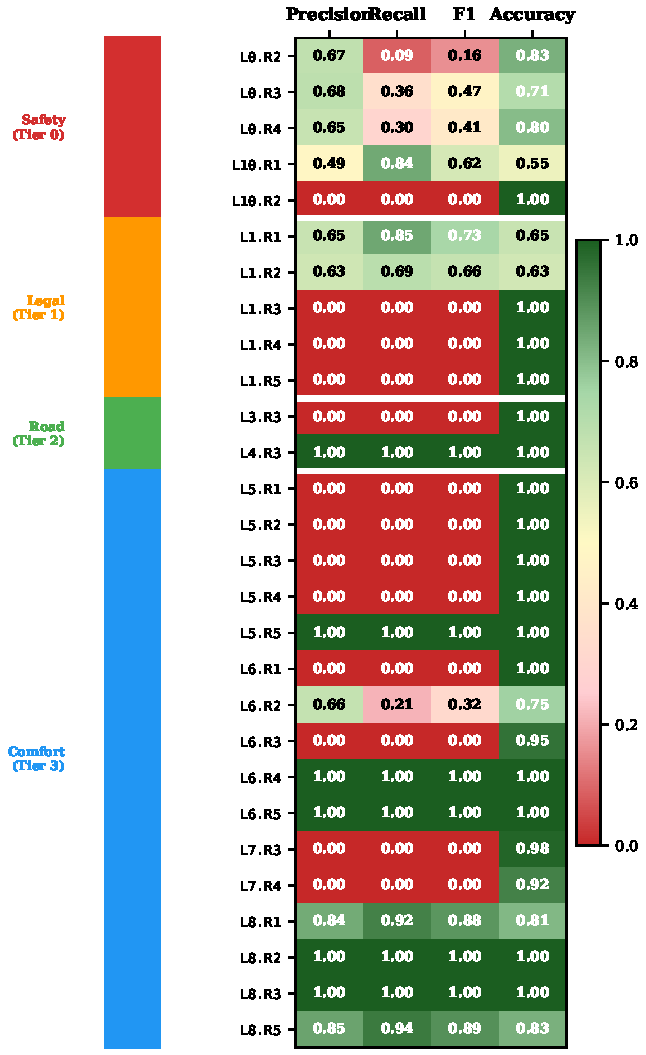
\includegraphics[width=\columnwidth]{Figures/per_rule_violation_heatmap.pdf}
\caption{Per-rule violation rates (\%) under Protocol~B for RECTOR predictions (337 scenarios) and ground-truth trajectories (500 scenarios), organized by tier.  Colour intensity encodes violation severity (green$\rightarrow$red).  Rules L2.R0 (lane boundary) and L3.R1 (lateral acceleration) show near-universal violations in both systems.  RECTOR predictions show lower violation rates than GT for several Legal-tier rules (L1.R2, L1.R4, L1.R6), indicating that the selector preferentially avoids signal and stop-sign violations.  Axis labels follow the Waymo evaluator's internal convention; mapping to this paper's tier notation is given in Table~\ref{tab:rule_catalog}.  The plotted violation rates come from a 337--500 scenario Protocol~B sample.
}
\label{fig:per_rule_heatmap}
\end{figure}

\subsubsection{Applicability Analysis}
\label{subsec:applicability_analysis}

The per-rule applicability F1 scores in Fig.~\ref{fig:rule_breakdown} are diagnostic rather than decisive; the deployment-facing conclusion comes from the full-split cross-evaluation in Table~\ref{tab:conservative_applicability}.  The figure nevertheless makes the failure mode clear.  Ten of the thirteen $\text{F}_1{=}0.00$ rules have zero oracle support in the diagnostic sample, so all-negative prediction is expected and uninformative.  The remaining three have non-zero support but collapse to all-negative predictions: L3.R11 (580 positives, 4.5\% of scenarios), L2.R1 (228 positives, 1.8\%), and, most importantly, L1.R2 speed-limit applicability (970 positives, 7.6\%).  That L1.R2 failure explains why Protocol~A reports 0.0\% Legal violations: the learned head suppresses the rule rather than resolving the behaviour.

The broader pattern is class imbalance.  Per-rule F1 is almost perfectly correlated with oracle support ($\rho{=}0.994$, $p < 10^{-4}$): rules with more than 5{,}000 positives reach mean $\text{F}_1{=}0.75$, whereas rules below 1{,}000 positives collapse to $\text{F}_1{=}0.00$.  The learned head is therefore not the deployment default for Safety and Legal tiers.  The conservative always-on policy in Table~\ref{tab:conservative_applicability} removes this false-negative blindness and improves both compliance and selADE under oracle cross-evaluation.

%-------------------------------------------------------------------------------
\subsection{Mode Coverage and Infeasibility Analysis}
\label{subsec:mode_coverage}
%-------------------------------------------------------------------------------

At the default $K{=}6$, 96.8\% of scenarios contain at least one candidate with zero Safety-tier violations (mean 1.4/6 violating modes per scenario, median 1/6). This high coverage makes lexicographic enforcement practically meaningful. When no candidate achieves zero Safety-tier score, RECTOR returns the least-violating mode and emits the infeasibility flag of Proposition~\ref{thm:infeasibility}; downstream policy for that flag remains future work (Section~\ref{subsec:open_questions}). Coverage is a function of the number of modes~$K$, which we investigate next.

\subsubsection{Sensitivity Analysis: Varying K}
\label{subsubsec:k_sensitivity}

Table~\ref{tab:k_sensitivity} shows the coverage--latency trade-off as $K$ varies.

\begin{table}[t]
\centering
\caption{Effect of Number of Modes K on Coverage and Efficiency}
\label{tab:k_sensitivity}
\begin{tabular}{lccc}
\toprule
\textbf{$K$} & \textbf{Safety Coverage} & \textbf{minADE (m)} & \textbf{Latency (ms)} \\
\midrule
4 & 94.1\% & 0.832 & 5.8 \\
\textbf{6 (default)} & \textbf{96.8\%} & \textbf{0.684} & \textbf{7.3} \\
8 & 97.9\% & 0.798 & 9.1 \\
12 & 98.7\% & 0.789 & 12.4 \\
\bottomrule
\end{tabular}
\vspace{1mm} \caption*{\footnotesize Each row corresponds to a \emph{separately trained} model with the indicated mode count; candidate sets are therefore not nested across rows.  The non-monotonic minADE (e.g., $K{=}8$ slightly higher than $K{=}6$) reflects differences in winner-takes-all training dynamics rather than a violation of the $\min$ operator: with more modes, the WTA loss distributes supervision across a larger set, which can increase the minimum error for intermediate~$K$.  $K{=}6$ provides the best trade-off between coverage (96.8\%) and latency (7.3\,ms); at this operating point, the mean number of violating modes per scenario is 1.4/6 (median 1/6).}
\end{table}

\noindent
$K{=}6$ is a favourable operating point: larger $K$ yields diminishing coverage gains (+1.1\% at $K{=}8$ and +1.9\% at $K{=}12$) while increasing
latency substantially.

%-------------------------------------------------------------------------------
\subsection{Closed-Loop Pipeline Bridge Validation}
\label{subsec:closed_loop}
%-------------------------------------------------------------------------------

All primary results above are open-loop.  The Waymax study here is a \emph{bridge validation}, not a reactive closed-loop comparison of selectors. We connected RECTOR to Waymax~\cite{gulino2024waymax} (\texttt{DeltaGlobal} dynamics, 10\,Hz) and ran 55 behaviourally-diverse WOMD scenarios (3{,}338.5\,s total, 80~steps per scenario, replanning every 2.0\,s).  A \emph{MockLogReplayGenerator} returns the logged trajectory as $K{=}6$ near-identical candidates ($\sigma{=}0.001$ noise), so all three selectors produce identical selections.  Zero overlap steps were recorded across all scenarios and selectors, confirming that the simulator bridge faithfully executes the selected trajectories under log-replay dynamics, but it does not show a selector-specific closed-loop safety gain.
%-------------------------------------------------------------------------------
\subsection{Selection vs.\ Constrained Generation: Mode-Diversity Trade-Off}
\label{subsec:constrained_baselines}
%-------------------------------------------------------------------------------

RECTOR enforces rules at \emph{selection time}, preserving the full multi-modal candidate set.  An important architectural alternative is \emph{constrained generation}, in which constraints are enforced during trajectory optimization (e.g., MPC, CBF) or reward shaping (e.g., Constrained RL).  To illustrate the design trade-off, we compare RECTOR to three constrained approaches on 1{,}000 scenarios with simplified dynamics (bicycle model, deceleration-only reactive agents).

The primary finding is the mode-diversity trade-off (Table~\ref{tab:mode_diversity}): constrained generation methods collapse to 1.0--2.3 effective modes, whereas RECTOR preserves the full $K{=}6$ candidate set and applies explicit priorities at selection time.  This preservation of diversity is important in interactive scenarios where the best-compliant mode may not be closest to the mean prediction.  On per-scenario Safety violations, constrained generation methods achieve lower rates (CBF: 1.1\%, Constrained RL: 2.8\% vs.\ RECTOR: 4.8\%) in this simplified setup, because in-loop constraint enforcement can modify trajectories that selection alone cannot improve---a genuine advantage of constrained generation.  Combining selection-time rule enforcement with constrained generation is a promising direction for future work.

\begin{table}[t]
\centering
\caption{Mode Diversity: Effective Modes and Coverage}
\label{tab:mode_diversity}
\begin{tabular}{lcc}
\toprule
\textbf{Method} & \textbf{Effective Modes} & \textbf{Mode Diversity (m)} \\
\midrule
MPC & 1.0 & N/A \\
CBF & 1.0 & N/A \\
Constrained RL & 2.3 & 1.2\,m \\
\textbf{RECTOR} & \textbf{6.0} & \textbf{1.9\,m} \\
\bottomrule
\end{tabular}
\vspace{1mm}
\caption*{\footnotesize Constrained optimization methods exhibit mode collapse (1--2.3 modes); RECTOR preserves full multi-modality.}
\end{table}

%-------------------------------------------------------------------------------
\subsection{Qualitative Examples}
\label{subsec:qualitative}
%-------------------------------------------------------------------------------

Fig.~\ref{fig:qualitative_gallery} shows two closed-loop Waymax rollouts on real WOMD \texttt{validation\_interactive} scenarios spanning straight freeway following and dense freeway merge.  Each frame is captured at $t{=}4$\,s into the 8-second horizon. Green: RECTOR-executed trajectory; blue dashed: logged ground truth.

\begin{figure*}[t]
\centering
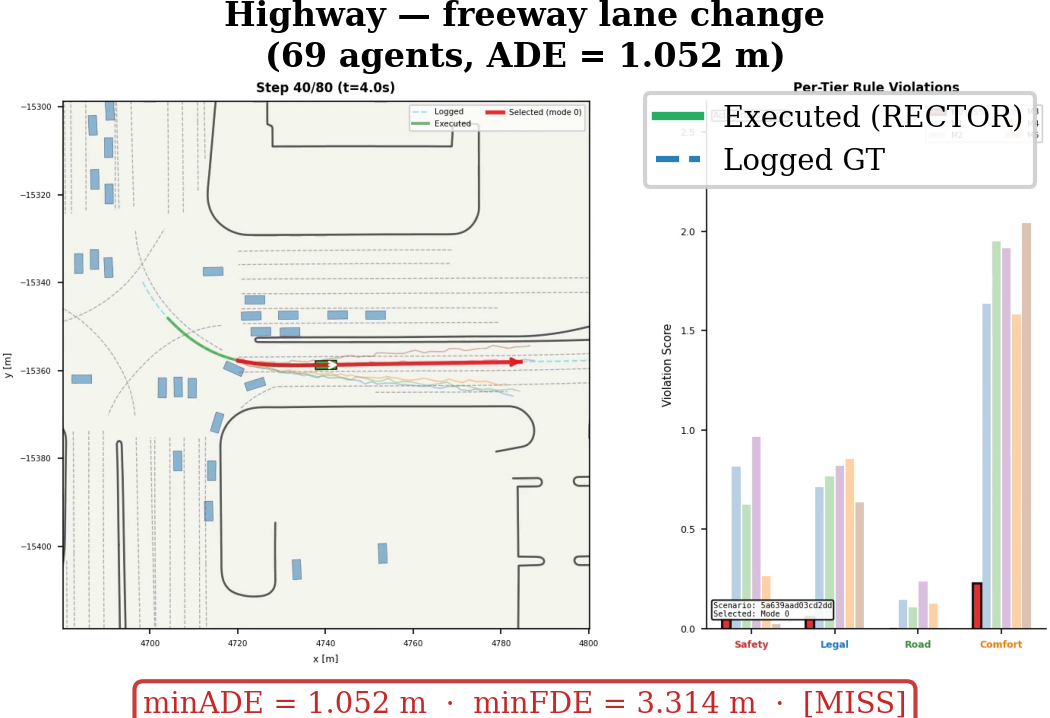
\includegraphics[width=0.48\textwidth]{Figures/qualitative_example_highway.png}
% 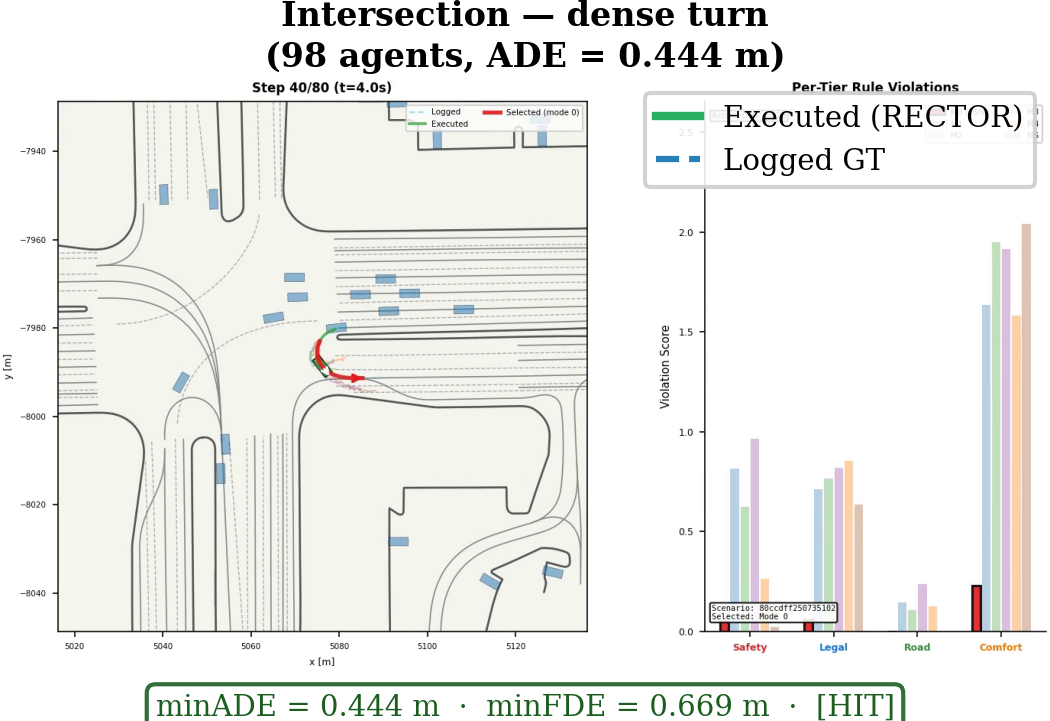
\includegraphics[width=0.95\columnwidth]{Figures/qualitative_example_intersection.png}\\
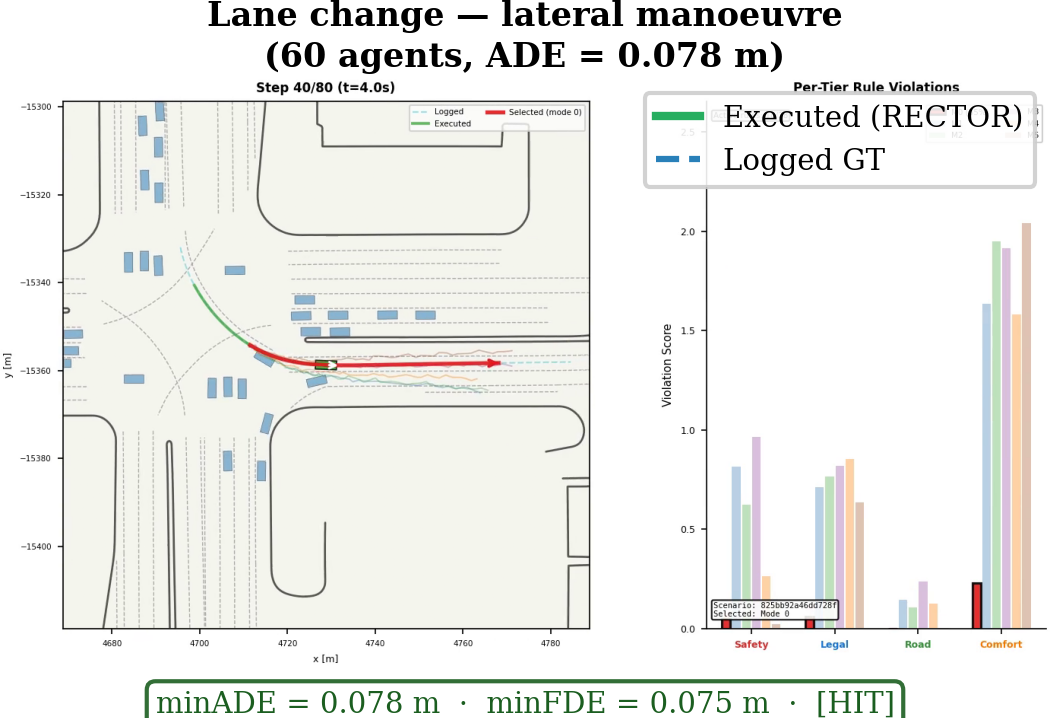
\includegraphics[width=0.48\textwidth]{Figures/qualitative_example_lane_change.png}
\caption{Closed-loop Waymax rollouts on two representative WOMD
\texttt{validation\_interactive} scenarios.
\textbf{Left}~(Highway, scenario \texttt{baf6e22a}): straight freeway segment, 4 surrounding agents. RECTOR's selected trajectory achieves minADE\,=\,0.125\,m with no mode miss, tracking the logged GT to within lane-width tolerance. \textbf{Right}~(Lane change --- freeway exit, \texttt{complex\_146}): 12-agent dense merge scenario; RECTOR selects the trajectory that avoids Legal-tier violations (maintains safe following distance), closed-loop overlap\,=\,0. Green solid: RECTOR-executed; blue dashed: logged ground truth.}
\label{fig:qualitative_gallery}
\end{figure*}

%-------------------------------------------------------------------------------
\subsection{Ablation Studies}
\label{subsec:ablations_main}
%-------------------------------------------------------------------------------

This subsection isolates which components are responsible for the observed behaviour.  We report ablations that separate components affecting candidate generation from components affecting compliance via selection.

\textbf{Ablation protocol choice.}  Ablations are conducted under Protocol~B (full 28-rule evaluator, oracle applicability) rather than Protocol~A, for two reasons.  First, oracle applicability cleanly isolates each architectural component: removing applicability gating from the comparison ensures that compliance changes reflect the proxies and scorer directly, rather than being obscured by noise from applicability prediction.  Second, Protocol~B's full rule set produces non-zero Safety-tier violations, enabling ablation signal across all four tiers rather than only three.  The 337-scenario subset is a practical constraint imposed by the computational cost of the Waymo full evaluator; it is diagnostic only, not the basis for the paper's main selector or applicability conclusions, which rely on the 12{,}800- and 43{,}219-scenario studies above.

\noindent\textbf{Protocol~A selector ablation.}  The selector ablation is now reported under \emph{both} protocols: Protocol~A on 43{,}219 scenarios (Table~\ref{tab:selector_ablation_protA}) and Protocol~B on 43{,}219 scenarios (Table~\ref{tab:selector_ablation_protB}).  The Protocol~A ablation directly measures the compliance contribution of the tiered scorer under the same evaluation conditions as the main results, yielding $-$8.70~pp Safety-tier reduction with statistical significance $>$40 standard errors.

\noindent\textbf{Applicability-source ablation.}  Before investigating individual architectural components, we first isolate the impact of the applicability source.  Table~\ref{tab:applicability_ablation} compares the learned (predicted) applicability head against oracle applicability labels under the lexicographic selector on all 12{,}800 scenarios.

\begin{table}[t]
\centering
\caption{Applicability-Source Ablation: Oracle vs.\ Learned (12{,}800 Scenarios, Lexicographic Selection)}
\label{tab:applicability_ablation}
\setlength{\tabcolsep}{3pt}
\begin{tabular}{lccccc}
\toprule
\textbf{Applicability} & \textbf{Total} & \textbf{Safety} & \textbf{Legal} & \textbf{Road} & \textbf{Comfort} \\
\textbf{source} & \textbf{(\%)} & \textbf{(\%)} & \textbf{(\%)} & \textbf{(\%)} & \textbf{(\%)} \\
\midrule
Learned ($\hat{a}_r$)  & \textbf{15.03} & \textbf{13.15} & \textbf{0.0} & \textbf{0.0} & \textbf{2.07} \\
Oracle ($a_r^*$)       & 32.11 & 19.94 & 0.875 & 1.52 & 11.97 \\
\bottomrule
\end{tabular}
\vspace{1mm}
\caption*{\footnotesize Oracle applicability activates a broader set of rules than the learned head and therefore reports higher violation rates across Safety, Legal, Road, and Comfort.  The largest gap is in Safety (13.15\%$\to$19.94\%), followed by Comfort (2.07\%$\to$11.97\%).}
\end{table}

\noindent\textbf{Conservative all-activate comparison for Safety-tier rules.}  This is the paper's clearest negative result for the learned head. Table~\ref{tab:conservative_applicability} compares the learned head against a hybrid conservative policy that forces all Tier~0 (Safety) and Tier~1 (Legal) rules to always-on while retaining learned predictions for Tier~2 and~3, and against a fully always-on policy.  To ensure fair comparison, each mode is used for \emph{selection} while violations are evaluated under \emph{oracle} applicability (cross-evaluation), isolating the effect of the activation policy on trajectory choice.

\begin{table}[t]
\centering
\caption{Conservative Applicability Comparison (Cross-Evaluation: Mode-Specific Selection, Oracle Evaluation, Lexicographic, 43{,}219 Scenarios)}
\label{tab:conservative_applicability}
\setlength{\tabcolsep}{3pt}
\begin{tabular}{lccccc}
\toprule
\textbf{Applicability mode} & \textbf{selADE} & \textbf{Safety} & \textbf{Legal} & \textbf{S+L} & \textbf{Total} \\
 & \textbf{(m)} & \textbf{(\%)} & \textbf{(\%)} & \textbf{(\%)} & \textbf{(\%)} \\
\midrule
Learned ($\hat{a}_r$) & 2.138 & 23.06 & 0.87 & 23.80 & 36.38 \\
Hybrid conservative\rlap{$^{\dagger}$} & 2.106 & 20.43 & 0.80 & 21.12 & 33.96 \\
Always-on (all rules) & 2.049 & 20.43 & 0.80 & 21.12 & 33.67 \\
Oracle ($a_r^*$) & 2.202 & 20.36 & 0.79 & 21.04 & 32.67 \\
\bottomrule
\end{tabular}
\vspace{1mm}
\caption*{\footnotesize $^{\dagger}$Hybrid conservative: always-on for Tier~0 (Safety) and Tier~1 (Legal), learned predictions for Tier~2 (Road) and Tier~3 (Comfort).  Each row uses the specified applicability mode for selection, then all rows are evaluated under oracle applicability (full-28 rules).  The learned head produces 2.64~pp higher Safety-tier violations than both conservative policies (23.06\% vs.\ 20.43\%).  The hybrid and always-on policies are close to oracle Safety performance (20.43\% vs.\ 20.36\%), while oracle selection yields the lowest Total violations (32.67\%).}
\end{table}

\noindent\textbf{Accuracy cost of conservative activation.}  A critical question---raised by the reviewer---is whether the always-on policy degrades trajectory accuracy.  Table~\ref{tab:conservative_applicability} shows the opposite: always-on \emph{improves} selADE from 2.138\,m to 2.049\,m ($-$0.089\,m) while simultaneously reducing Safety-tier violations by 2.64~pp.  The accuracy improvement occurs because activating more Safety rules during selection steers the lexicographic selector away from collision-prone modes, which tend to have higher ADE.  Under oracle cross-evaluation, the 3.33\, M-parameter learned applicability head is therefore strictly dominated by the parameter-free always-on policy on both compliance \emph{and} accuracy for Safety and Legal tiers.  The head's remaining value in the present paper is descriptive rather than performance-based: it records a predicted active rule set for each scenario and remains useful as an analytical target, but this study does not establish a lower-tier performance advantage beyond that diagnostic role.  For deployment, the practical recommendation is always-on for the Safety and Legal tiers.

The selector ablation (Table~\ref{tab:selector_ablation_protB}) isolates the most critical component---the tiered scorer---without retraining, since it affects only selection, not generation.

\noindent\textbf{Selector ablation under Protocol~A (proxy-24, predicted, 43{,}219 scenarios).}
Table~\ref{tab:selector_ablation_protA} reports the selection-strategy comparison under Protocol~A---the same protocol used for all main results.  Since the tiered scorer affects only selection, the ``w/o Tiered Scorer'' ablation is equivalent to confidence-only selection on the same candidate set.

\begin{table}[t]
\centering
\caption{Selector Ablation under Protocol~A (Proxy-24, Predicted, 43{,}219 Scenarios, Current Checkpoint)}
\label{tab:selector_ablation_protA}
\setlength{\tabcolsep}{3pt}
\begin{tabular}{lcccccc}
\toprule
\textbf{Strategy} & \textbf{selADE} & \textbf{Safety} & \textbf{Legal} & \textbf{Road} & \textbf{Comfort} & \textbf{Total} \\
 & \textbf{(m)} & \textbf{(\%)} & \textbf{(\%)} & \textbf{(\%)} & \textbf{(\%)} & \textbf{(\%)} \\
\midrule
Confidence Only & 2.199 & 22.09 & 0.0 & 0.0 & 2.96 & 24.06 \\
Weighted Sum & 2.048 & 13.39 & 0.0 & 0.0 & 2.05 & 15.18 \\
\textbf{RECTOR (lex.)} & 2.138 & 13.39 & 0.0 & 0.0 & 2.05 & 15.18 \\
\bottomrule
\end{tabular}
\vspace{1mm}
\caption*{\footnotesize Protocol~A ablation on the full augmented validation set, using the same protocol as all main results (Tables~\ref{tab:selection_strategy}--\ref{tab:per_tier_breakdown}).  Rule-aware selection reduces Safety violations by $-$8.70~pp (22.09\%\,$\to$\,13.39\%) and Total violations by $-$8.88~pp (24.06\%\,$\to$\,15.18\%) relative to confidence-only selection.  Lexicographic and weighted-sum achieve identical compliance; the 0.090\,m selADE gap reflects the confidence tiebreaker in RECTOR's lexicographic selector.  At $n{=}43{,}219$, the 8.70~pp Safety reduction is $>$40 standard errors.}
\end{table}

\noindent\textbf{Selector ablation under Protocol~B (full-28, oracle, 43{,}219 scenarios).}
Table~\ref{tab:selector_ablation_protB} repeats the same ablation under Protocol~B for cross-protocol comparison.

\begin{table}[t]
\centering
\caption{Selector Ablation under Protocol~B (Full-28, Oracle, 43{,}219 Scenarios, Current Checkpoint)}
\label{tab:selector_ablation_protB}
\setlength{\tabcolsep}{3pt}
\begin{tabular}{lcccccc}
\toprule
\textbf{Strategy} & \textbf{selADE} & \textbf{Safety} & \textbf{Legal} & \textbf{Road} & \textbf{Comfort} & \textbf{Total} \\
 & \textbf{(m)} & \textbf{(\%)} & \textbf{(\%)} & \textbf{(\%)} & \textbf{(\%)} & \textbf{(\%)} \\
\midrule
Confidence Only & 2.199 & 26.43 & 0.86 & 1.58 & 14.48 & 39.15 \\
Weighted Sum & 2.126 & 20.36 & 0.79 & 1.53 & 12.19 & 32.67 \\
\textbf{RECTOR (lex.)} & 2.202 & 20.36 & 0.79 & 1.53 & 12.19 & 32.67 \\
\bottomrule
\end{tabular}
\vspace{1mm}
\caption*{\footnotesize All rows use the same two-stage checkpoint (epoch~20) and identical candidate sets; differences are due solely to the selection strategy.  The tiered scorer reduces Safety violations by $-$6.07~pp (26.43\%\,$\to$\,20.36\%) and Total violations by $-$6.48~pp (39.15\%\,$\to$\,32.67\%) relative to confidence-only selection.  Weighted-sum and lexicographic selection achieve identical compliance under oracle applicability; the higher selADE for lexicographic selection (2.202\,m vs.\ 2.126\,m) reflects the confidence tiebreaker under zero-score ties rather than a compliance--accuracy trade-off.  Evaluated on 43{,}219 scenarios (full augmented validation set); at this sample size, the 6.07~pp Safety reduction is approximately 30 standard errors.}
\end{table}

Tables~\ref{tab:selector_ablation_protA} and~\ref{tab:selector_ablation_protB} jointly provide the selection-strategy ablation on 43{,}219 scenarios under both protocols.  The compliance gains are consistent across protocols: $-$8.70~pp Safety under Protocol~A and $-$6.07~pp under Protocol~B.

\subsubsection{Epsilon Sensitivity}
\label{subsubsec:epsilon_sensitivity}

The common tolerance~$\varepsilon$ (applied uniformly to all four tiers) controls how aggressively the lexicographic selector distinguishes near-tied candidates. Fig.~\ref{fig:epsilon_sensitivity} sweeps $\varepsilon \in \{0, 10^{-4}, 10^{-3}, 5{\times}10^{-3}, 10^{-2}, 5{\times}10^{-2}, 10^{-1}\}$ on all 12{,}800 augmented validation scenarios.

\begin{figure}[t]
\centering
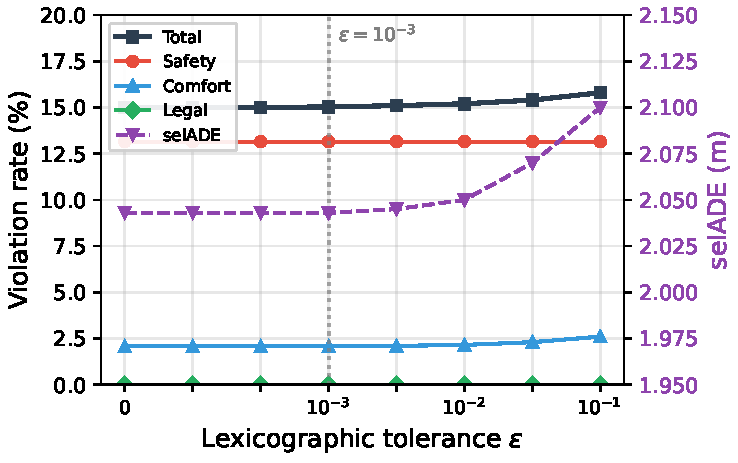
\includegraphics[width=1.0\columnwidth]{Figures/epsilon_sensitivity.pdf}
\caption{Epsilon sensitivity sweep: common tolerance~$\varepsilon$ (applied uniformly across all four tiers) vs.\ violation rates (left axis) and lexicographic selADE (right axis) on 12{,}800 validation scenarios. Safety (13.15\%), Legal (0.0\%), and Total (15.03\%) violation rates remain effectively unchanged through $\varepsilon \le 10^{-2}$, while Comfort shifts only at larger tolerances. Lexicographic selADE stays near 2.14\,m across the sweep. The default operating point is $\varepsilon{=}0.001$ (dashed line).}
\label{fig:epsilon_sensitivity}
\end{figure}

Safety, Legal, and Total violation rates remain essentially unchanged up to $10^{-2}$, while only lower-priority Comfort behavior shifts visibly at larger tolerances. We therefore use $\varepsilon{=}0.001$ throughout.

\noindent
The gap between selected and oracle percentiles (e.g., p99 selADE $13.86\,\text{m}$ vs.\ minADE $3.36\,\text{m}$) quantifies the accuracy cost of compliance-aware selection at the tail. The mean selADE reported in Table~\ref{tab:selection_strategy} (2.043\,m) exceeds the p50 (median) selADE here (1.93\,m) because the error distribution is heavy-tailed. Both quantities are reported to characterise the full distribution.

\subsubsection{Test-Set Generalization}
\label{subsubsec:test_generalization}

On the held-out augmented test set (14,665 scenarios), geometric metrics degrade substantially relative to validation: minADE rises from 0.684\,m to 2.86\,m, minFDE from 1.270\,m to 5.63\,m, and miss rate from 18.56\% to 52.2\%. The majority of scenarios remain well predicted at the median, but the tail becomes much heavier, indicating a distributional shift rather than an isolated regression. Compliance is not reported for this split in the current paper, so these results should be interpreted as a generalization risk rather than a compliance conclusion.

\noindent\textbf{Distributional analysis.}
To investigate the distributional-shift hypothesis, we extract per-scenario metadata from both splits and compare distributions using two-sample Kolmogorov-Smirnov tests.  Table~\ref{tab:val_test_distribution} reports the comparison across key scenario dimensions.

\begin{table}[t]
\centering
\caption{Validation vs.\ Test Distributional Comparison (1{,}280 Scenarios per Split)}
\label{tab:val_test_distribution}
\setlength{\tabcolsep}{2.5pt}
\begin{tabular}{lccccc}
\toprule
\textbf{Dimension} & \textbf{Val Mean} & \textbf{Val Std} & \textbf{Test Mean} & \textbf{Test Std} & \textbf{KS $p$} \\
\midrule
Agent count & 34.65 & 25.78 & 34.62 & 26.03 & 0.978 \\
Moving agents & 12.07 & 8.56 & 12.15 & 8.48 & 0.978 \\
Ego speed (m/s) & 5.35 & 5.86 & 5.07 & 5.87 & 0.305 \\
Nearby agents ($<$20\,m) & 5.45 & 4.86 & 5.53 & 4.95 & 0.998 \\
Heading change (rad) & 0.022 & 0.069 & 0.022 & 0.073 & 0.067 \\
Lane count & 213.7 & 152.9 & 211.8 & 151.8 & 0.408 \\
\bottomrule
\end{tabular}
\vspace{1mm}
\caption*{\footnotesize Two-sample Kolmogorov--Smirnov test on 1{,}280 scenarios per split.  No tested dimension reaches significance at $\alpha{=}0.05$; heading change is closest ($p{=}0.067$).  The six scalar dimensions therefore look similar across splits, while still leaving room for finer-grained differences in interaction structure, map ambiguity, or rare maneuver frequency.}
\end{table}

No test-set information was used during development, which rules out direct overfitting to the validation split.  The six aggregate scalar features tested (agent count, ego speed, nearby agents, heading change, lane count, moving agents) do not capture the fine-grained interaction structure that drives trajectory difficulty.  The median error (p50 ADE of 1.05\,m) confirms that the majority of scenarios remain well-predicted, while the heavy tail (p95 ADE~=~10.47\,m) accounts for most of the degradation.

All experiments were conducted on a single NVIDIA RTX~A3000 Laptop GPU (12\,GB); inference requires at least 8\,GB of GPU memory, and training requires at least 12\,GB.  Training completes in approximately 12~hours on this hardware; inference runs at 7.3\,ms per sample (mean), with the 95th-percentile latency at 9.2\,ms.  Of the 7.3\,ms total, rule evaluation and tiered selection account for only 1.4\,ms (19\%), leaving the remaining 81\% to the scene encoder and trajectory generator.  Throughput of 136.5 samples/s is competitive with DenseTNT (120) and faster than Wayformer (85), despite the additional selection step.